How deep do particles penetrate the detector material? For every combination of projectile and
target, we can only \ldots a mean depth of penetration. The loss of energy of a particle in
dependence of the penetration depth can be described by the Bragg curve. The projectile slows down
when penetrating into matter and the loss of energy increases (Bethe-Bloch). We obtain the range $R$
by integrating  the loss of enegy over the distance, where $\frac{dE}{dx}$ is a function of $E$. For
ionising radiation there is a particular high density of deposited energy  at the end of the range
because of $\frac{1}{\beta^2}$ (dependence).

\[dE= \frac{dE}{dx}(E)dx~~~~~~~~~~\Rightarrow~~~~~~~~~~dx
=\frac{dE}{dE/dx}~~~~~~~~~~\Rightarrow~~~~~~~~~~ R=\int_{E_c}^{M} \frac{dE}{dE/dx}  \]

The highest loss of energy is occurs at the end of the track (Bragg peak).

\begin{figure}[htbp]
	\begin{minipage}[b]{0.5\textwidth}
		\begin{figure}[H]
		\centering
		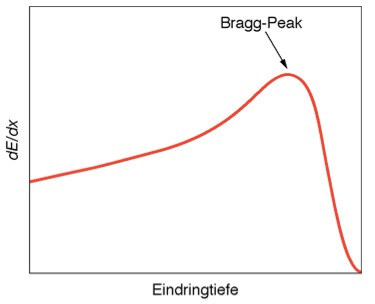
\includegraphics[width=\textwidth]{bragg.jpg}
		\end{figure}
	\end{minipage}
	\hfill
	\begin{minipage}[b]{0.5\textwidth}
		\begin{figure}[H]
		\centering
		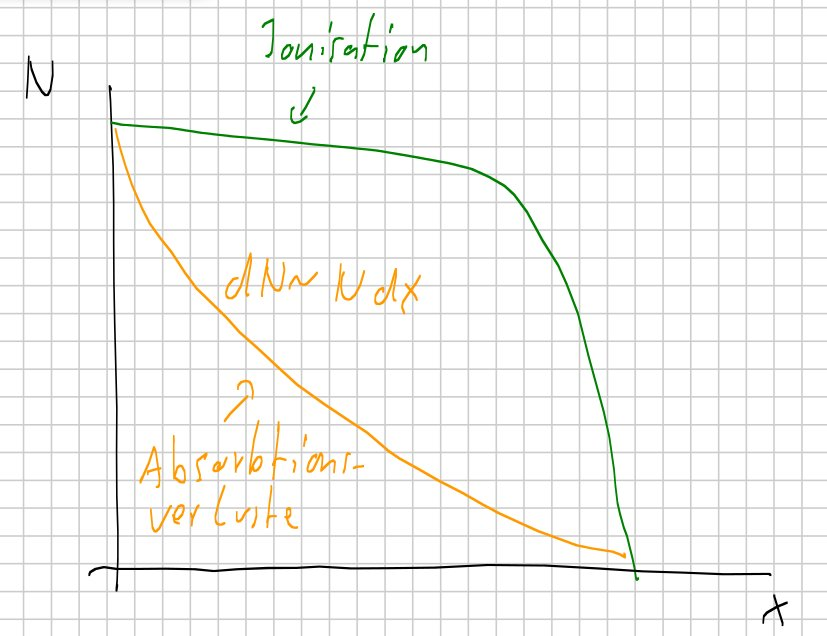
\includegraphics[width=\textwidth]{expabfall.jpg}
		\end{figure}
	\end{minipage}
	\caption{b}
	\label{rekristall} 
\end{figure}